\section{Iteration loop}\label{iteration-loop}

In section \ref{mandelbrot-set} there was mentioned that fractals are calculated
by repeating inside an iteration loop. The loop is terminated when the calculated
number of iterations equals to \emph{maxiter} or the bailout condition is reached.
In this section the calculations inside this loop will be explained.

\subsection{Single formula fractals}\label{single-formula-fractals}

The simplest 3D fractals are calculated using single fractal formula which is
build from many equations and conditions. These equations can be modifications
of Mandelbrot Set equation or can be different mathematical equations with
several conditions.

Below there are 3 examples of fractals formulas with C language code

\subsubsection{Mandelbulb Power 2}\index{Mandelbulb} \nopagebreak

This formula is modified Mandelbrot Set equation, expanded to \nth{3} dimension.
Cross section at $ z_z = 0 $ looks exactly the same as Mandelbrot Set.
\nopagebreak

\begin{tabular}{l l}
	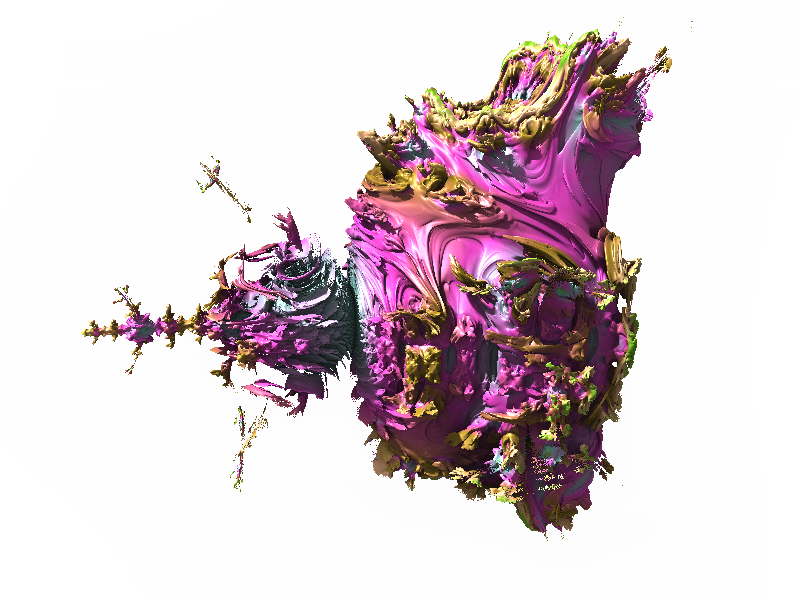
\includegraphics[width=0.3\linewidth]{img/manual/media/formula_mandelbulb_power_2}	
	& 
	\begin{minipage}[b]{0.5\linewidth}
	    \lstinputlisting[caption={Formula > Mandelbulb Power 2}]{code/formula_mandelbulb_power_2.cpp}
	\end{minipage}
\end{tabular} 

\subsubsection{Menger Sponge}\index{Menger Sponge} \nopagebreak

This formula is Iterated Function System (IFS). It contains several
transformations where some of them are conditional. \nopagebreak

\begin{tabular}{l l}
    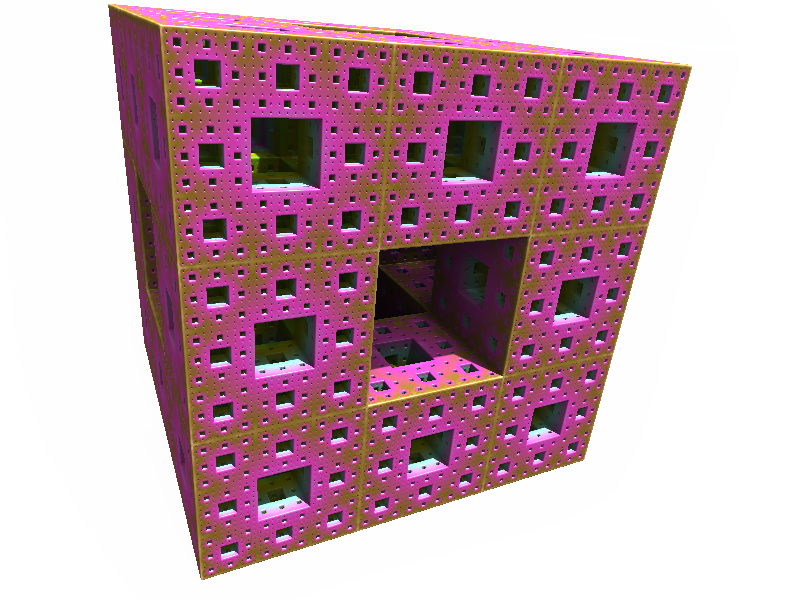
\includegraphics[width=0.3\linewidth]{img/manual/media/formula_menger_sponge.png}
	& 
	\begin{minipage}[b]{0.5\linewidth}
	    \lstinputlisting[caption={Formula > Menger Sponge}]{code/formula_menger_sponge.cpp}
	\end{minipage}
\end{tabular} 

\subsubsection{Box Fold Bulb Pow 2}
\nopagebreak

This formula is a set of different transforms and equations. It's a good example
which shows that fractal formula can be much more complicated than
\emph{Mandelbrot Set}.

First part is ``box fold''\index{transform!box fold} transform which do
transformations based on box walls. Second part is ``spherical
fold''\index{transform!spherical fold} which do transformations based on sphere.
The end of formula is the same as \emph{Mandelbulb Power 2}.\nopagebreak

\begin{tabular}{l l}
	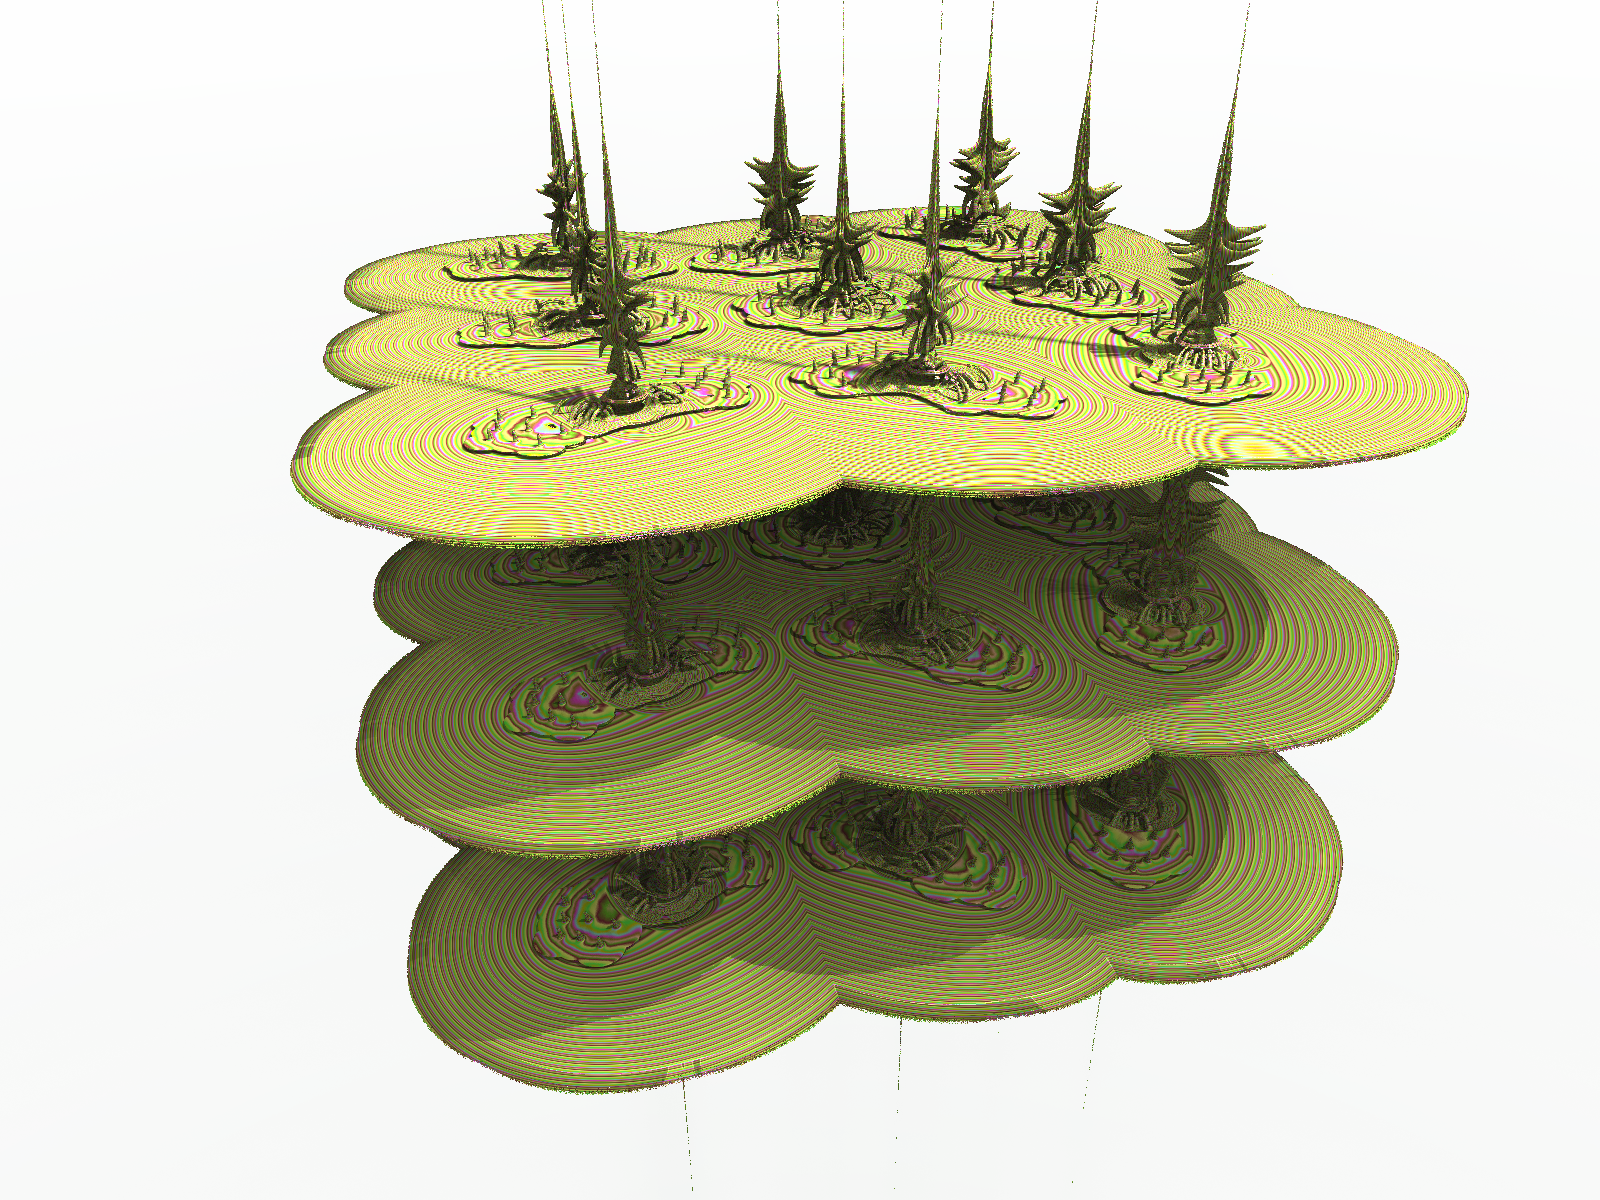
\includegraphics[width=0.3\linewidth]{img/manual/media/formula_box_fold_pwr2.png}	
	& 
	\begin{minipage}[b]{0.5\linewidth}
	    \lstinputlisting[caption={Formula > Box fold Power 2}]{code/formula_box_fold_pwr2.cpp}
	\end{minipage}
\end{tabular} 

\subsubsection{Processing of single formula fractals}

Single formula fractals are processed in a simple way. The calculation of the fractal
formulas is repeated several times like it is shown in the following two
diagrams:\nolinebreak \nopagebreak

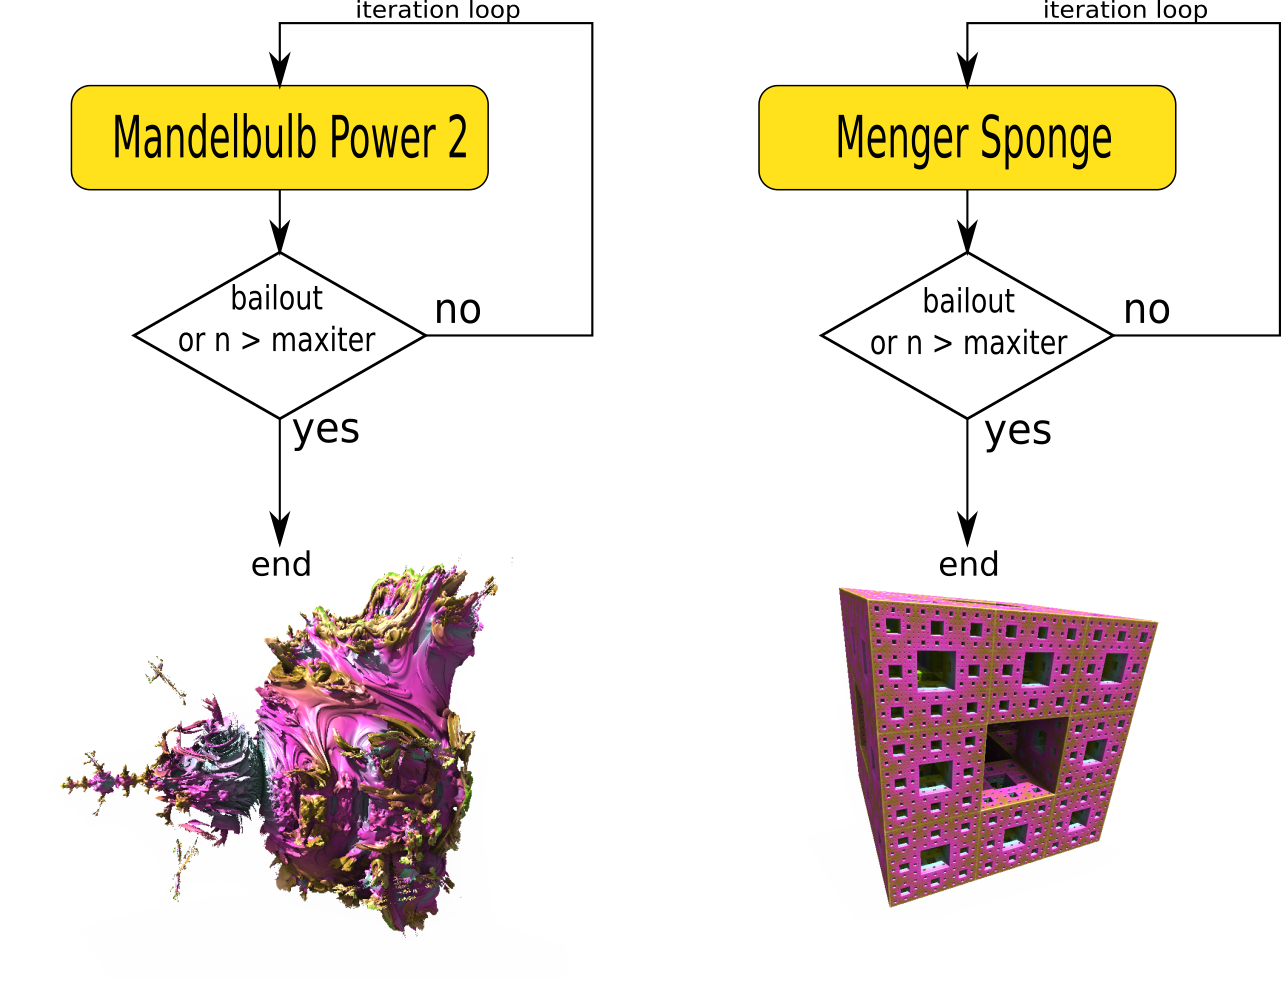
\includegraphics[width=\linewidth]{img/manual/media/iteration_loops.png}

When the calculation of the iteration loop finishes the result value of \emph{z} is
used to estimate the distance to the fractal body and to calculate the color of the surface.

\subsection{Hybrid fractals}\index{fractal!hybrid}

It is possible to mix different fractal formulas by alternating their use in the iteration loop.
This way new fractal shapes can be achieved. These fractal combinations are named \emph{hybrid fractals}. 
In the Mandelbulber program there are already many different fractal formulas available which give the user 
the opportunity to use a vast variety of shapes.

\subsubsection{Iteration loop of hybrid fractals}

In general hybrid fractals are calculated in the same way as regular fractals.
The calculation consists of iteration loop, \emph{maxiter} and \emph{bailout} condition. The
difference is in the body of the iteration loop: Instead of one fractal formula there
can be used a different fractal formula in every iteration. The defined
sequence decides in which iteration which formula will be used as the calculation step.
How the sequence will work depends on the following selections:
\begin{itemize}
    \item Which fractal formulas are selected in formula slots
	\item How many iterations are assigned to each formula
	\item Range of iteration numbers where formula will be used
	\item From which fractal slot the sequence will be repeated
\end{itemize}

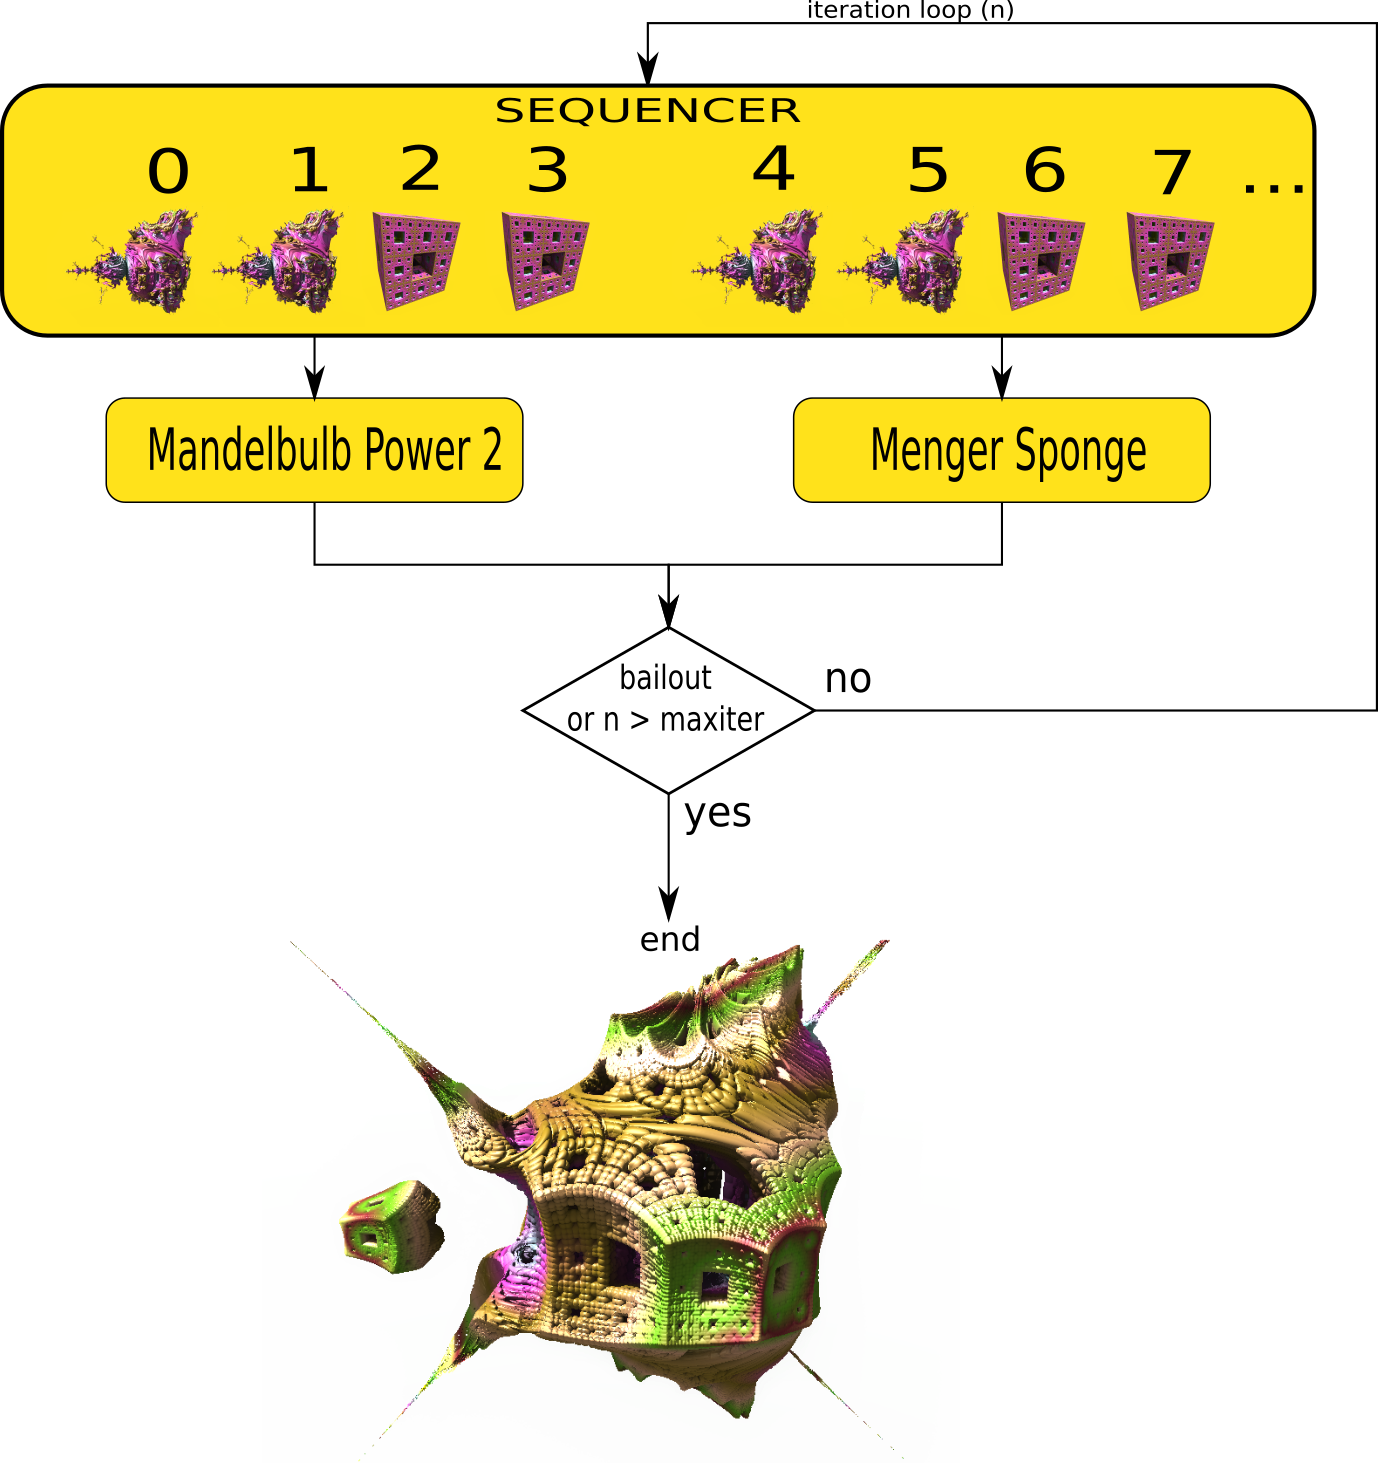
\includegraphics[width=\linewidth]{img/manual/media/iteration_loop_hybrid.png}

In Mandelbulber it is possible to define nine different fractal formulas which
ca be alternated. Each formula is configured in a separate slot (tab).

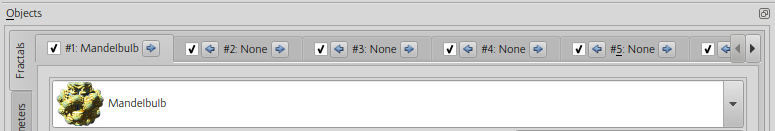
\includegraphics[width=\linewidth]{img/manual/media/fractal_tabs.png}

By default it is possible to setup the fractal formula in the first slot only,
because the program works in single fractal formula mode. There are two ways to
enable hybrid fractals:
\begin{itemize}
    \item Click in any slot with a number higher than one. The program will ask if you want to
	    enable hybrid fractals or boolean mode. Select \emph{Enable hybrid fractals}
	\item Go to \emph{Objects} / \emph{Hybrid} tab. Tick \emph{Enable hybrid fractals} checkbox.
\end{itemize}

After that you can switch to any slot and define fractal formulas in each slot
(if needed) like it's shown below:

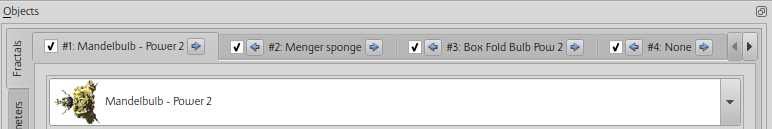
\includegraphics[width=\linewidth]{img/manual/media/fractal_tabs_with_defined_fractals.png}

Here \emph{Mandelbulb - Power 2} is selected in slot \#1, \emph{Menger Sponge}
in slot \#2 and \emph{Box Fold Bulb Pow 2} in slot \#3. These formulas will be
used in the next examples.

\subsubsection{One iteration for each slot}

The simplest way how hybrid fractal can be defined is to use each fractal
formula for only one iteration in the looped sequence.

In the example below, the sequence consists of one \emph{Mandelbulb - Power 2}, one \emph{Menger Sponge} and
one \emph{Box Fold Bulb Pow 2}. The length of the sequence is three, so by every three
iterations the sequencer repeats with the first slot:

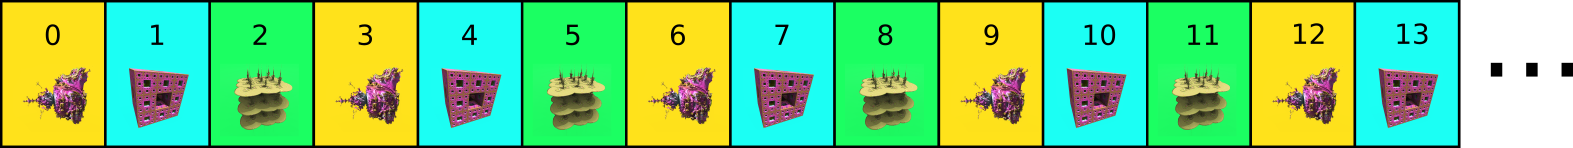
\includegraphics[width=\linewidth]{img/manual/media/iteration_loop_hybrid_sequence_1.png}

This sequence gives the following shape which is a mix of properties of all 3
formulas: \nopagebreak

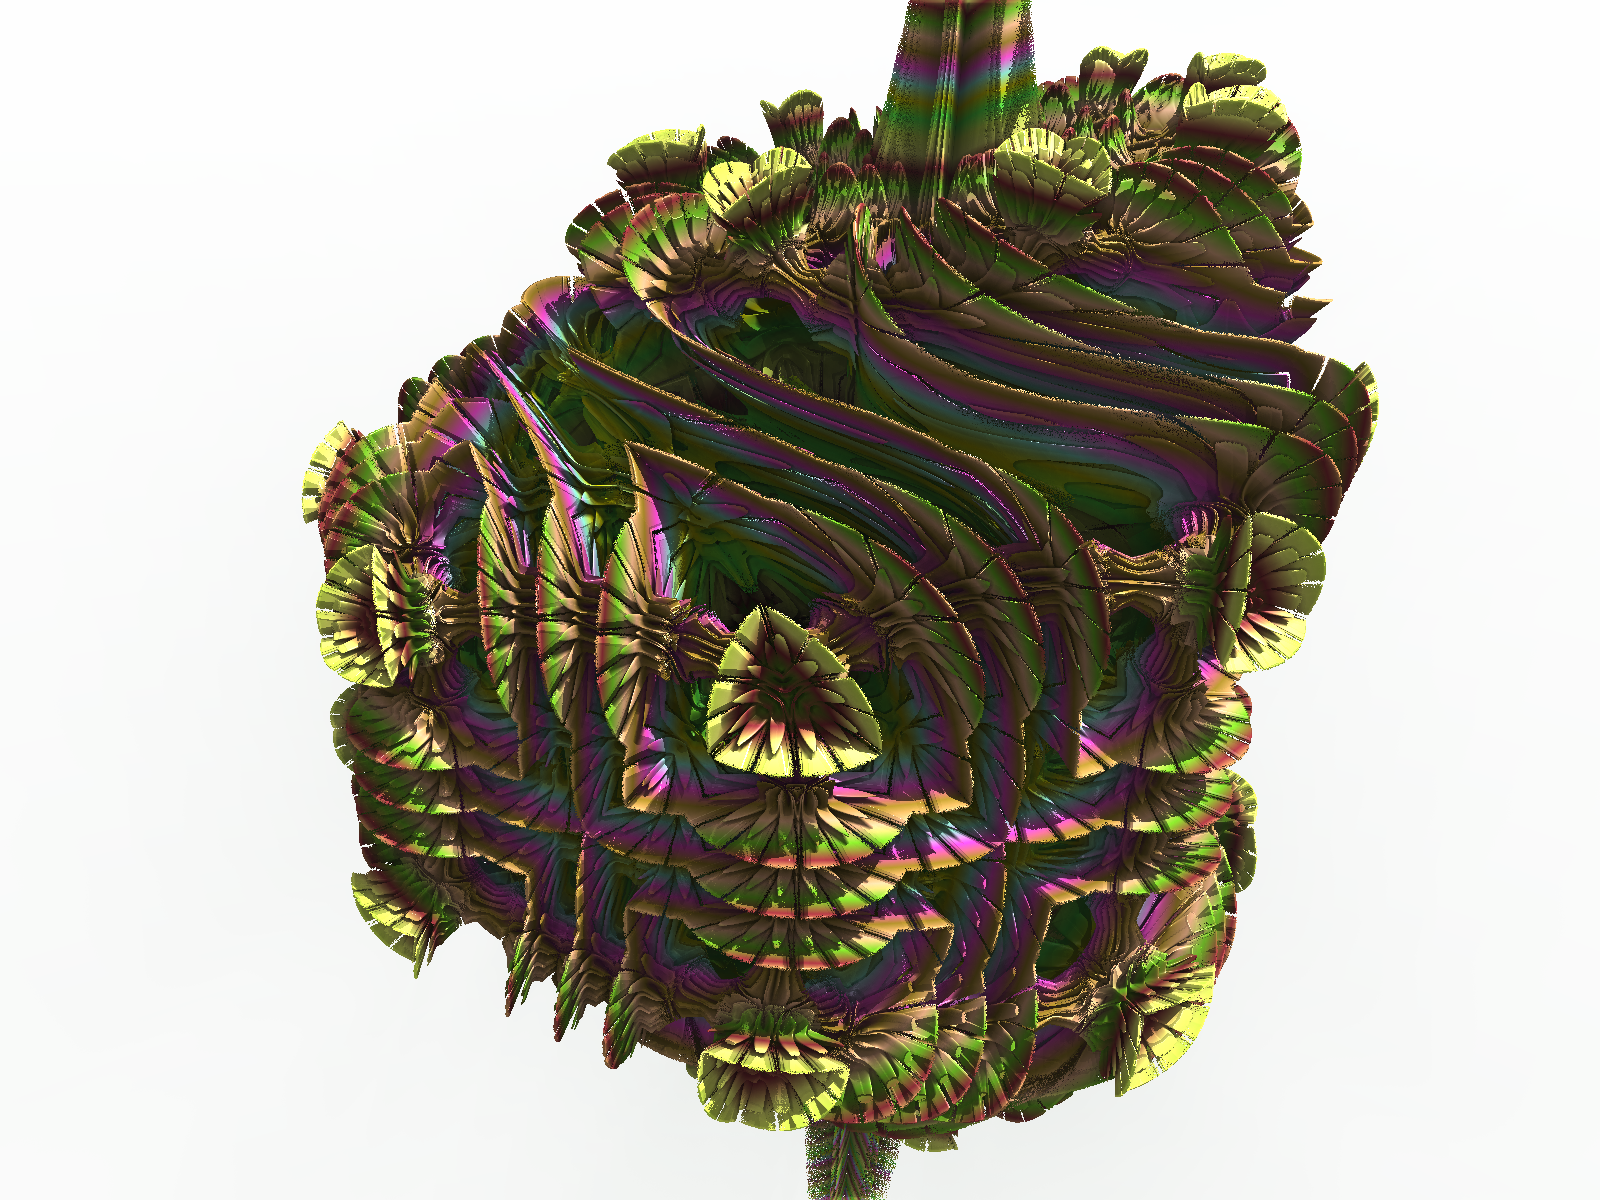
\includegraphics[width=0.7\linewidth]{img/manual/media/hybrid_sequence_example_1.png}

Because in the first iteration (slot \#1) \emph{Mandelbulb - Power 2} is used, the general shape
of the fractal is a little similar to \emph{Mandelbulb - Power 2}.

In the next iteration the \emph{Menger Sponge} formula is used. A single iteration
of this formula produces this shape:

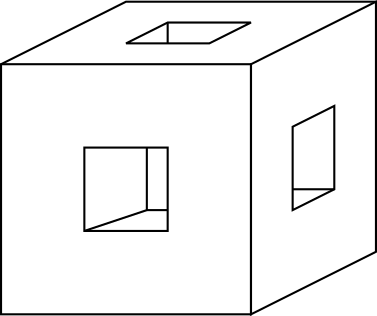
\includegraphics[width=0.2\linewidth]{img/manual/media/single_iteration_of_menger_sponge.png}

Some properties of this shape are transferred to the generated shape of the hybrid fractal:

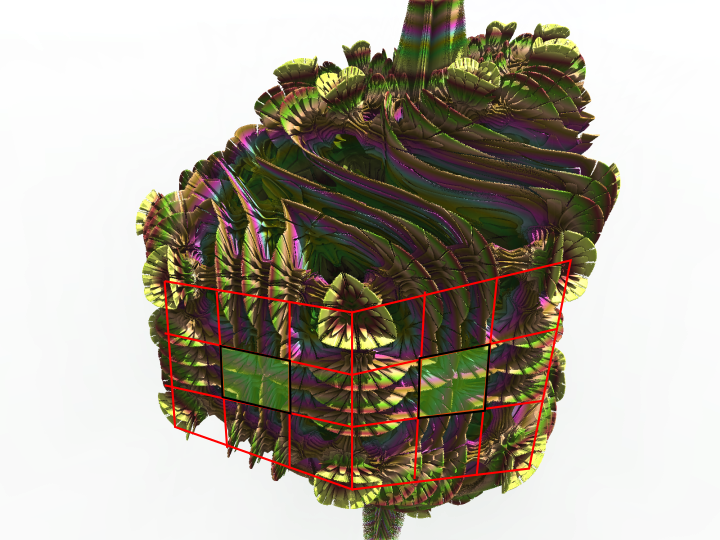
\includegraphics[width=0.5\linewidth]{img/manual/media/single_iteration_of_menger_sponge_hybrid.png}

The Menger sponge shape is distorted, because \emph{Mandelbulb - Power 2} has
already deformed the space.

The third formula \emph{Box Fold Bulb Pow 2} adds leaf-like features to the shape:

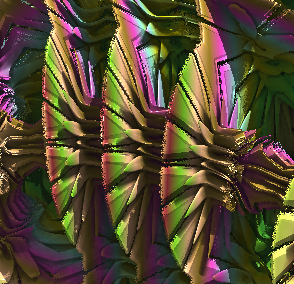
\includegraphics[width=0.4\linewidth]{img/manual/media/hybrid_sequence_example_1_leaf_shapes.png}

\subsubsection{More iterations for each slot}

In each slot it is configurable how many times the fractal formula will be used in the sequence.
On the tab for the given fractal there is parameter \emph{Iterations}.
By default it is set to 1. If this value was increased to 2 on the first and the second tab,
the sequence of formulas will look as following:\label{two-iterations-per-slot}

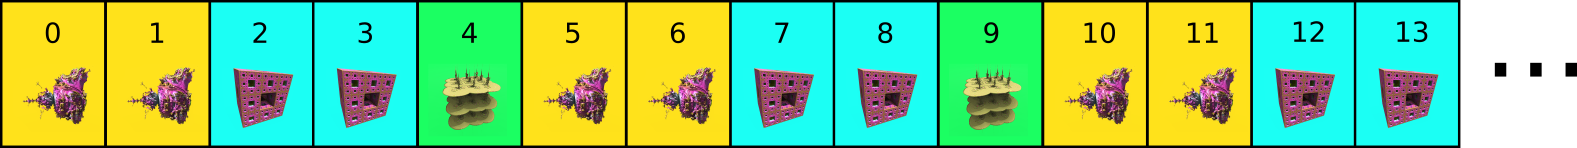
\includegraphics[width=\linewidth]{img/manual/media/iteration_loop_hybrid_sequence_2.png}

The first and the second formula is repeated twice and the third only once.
The fractal will get following shape:

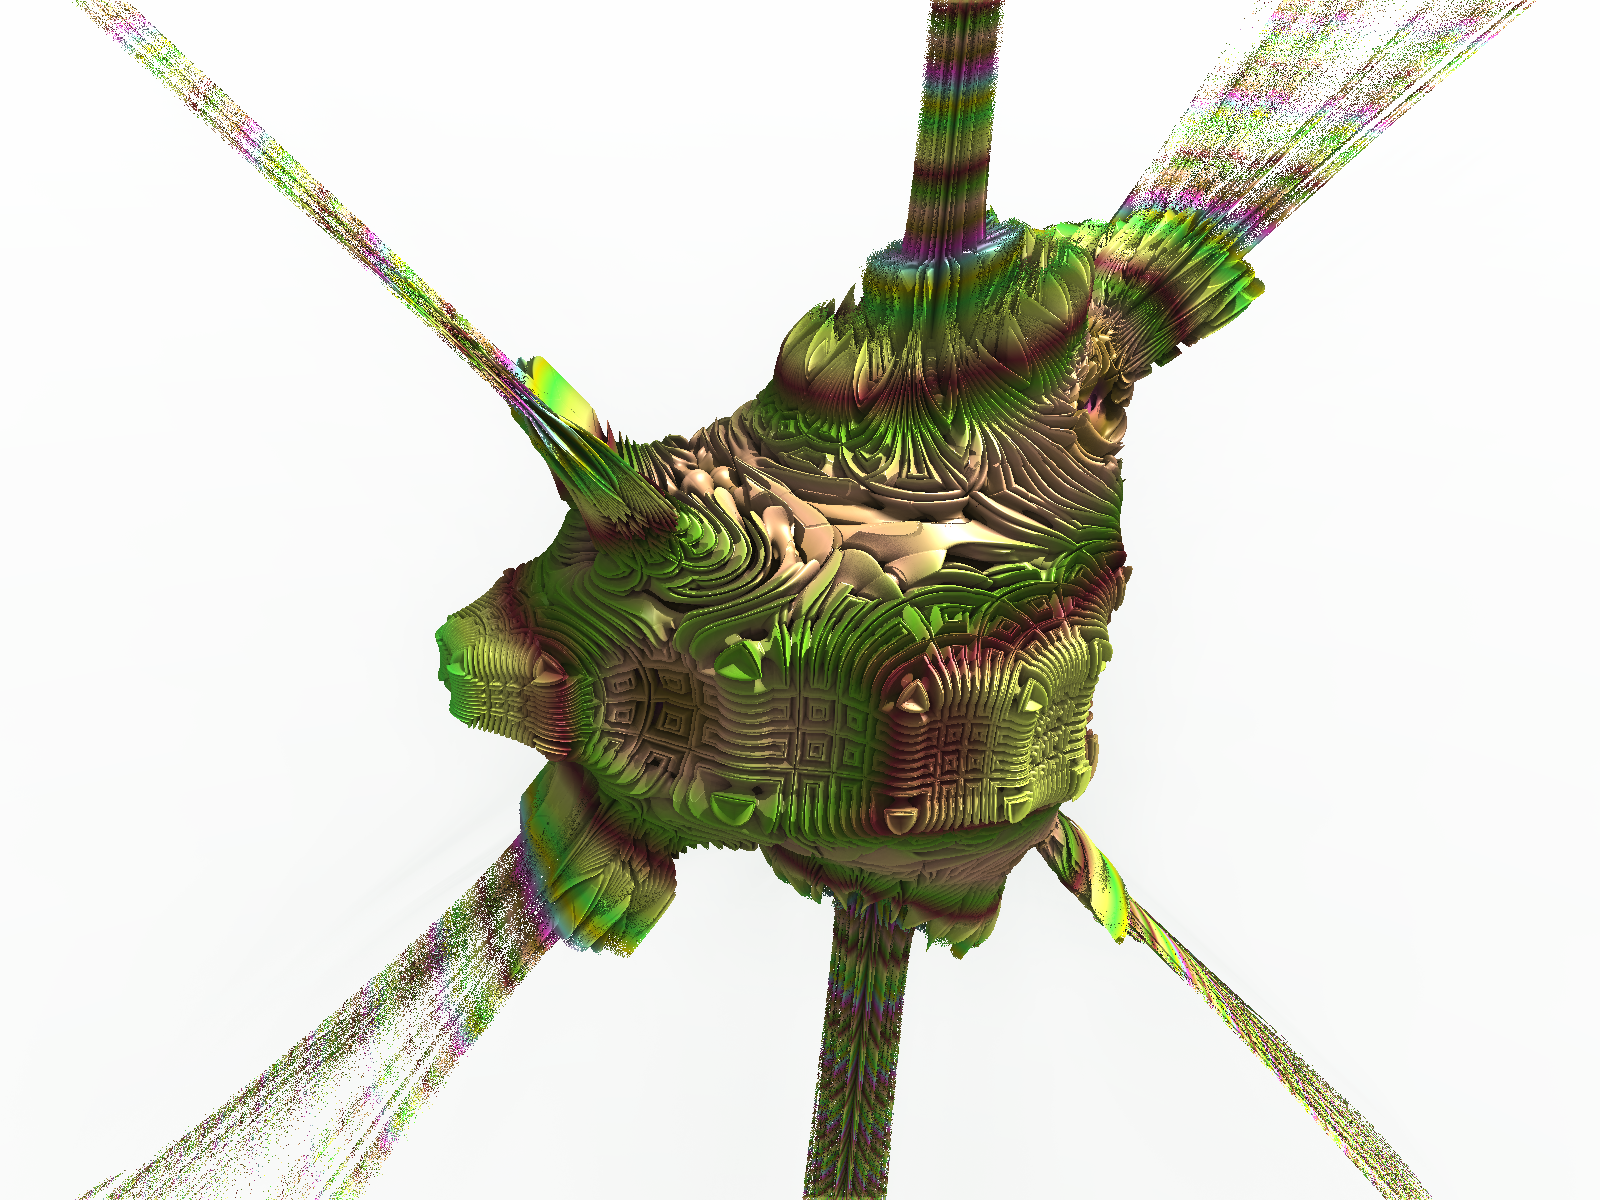
\includegraphics[width=0.7\linewidth]{img/manual/media/hybrid_sequence_example_2.png}

Because \emph{Mandelbulb - Power 2} has two iterations at the beginning, the shape of this formula is more visible.

If the parameter \emph{Iterations} on the second tab is set to 10,
then the \emph{Menger Sponge} formula is used from iteration 2 to iteration 11.

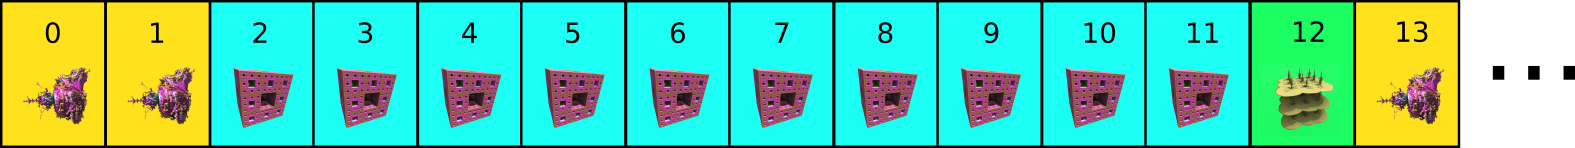
\includegraphics[width=\linewidth]{img/manual/media/iteration_loop_hybrid_sequence_3.png}

Like before the initial shape is defined by the first two iterations of \emph{Mandelbulb - Power 2},
but the high number of \emph{Menger Sponge} iterations makes \emph{Menger Sponge} features very well visible.

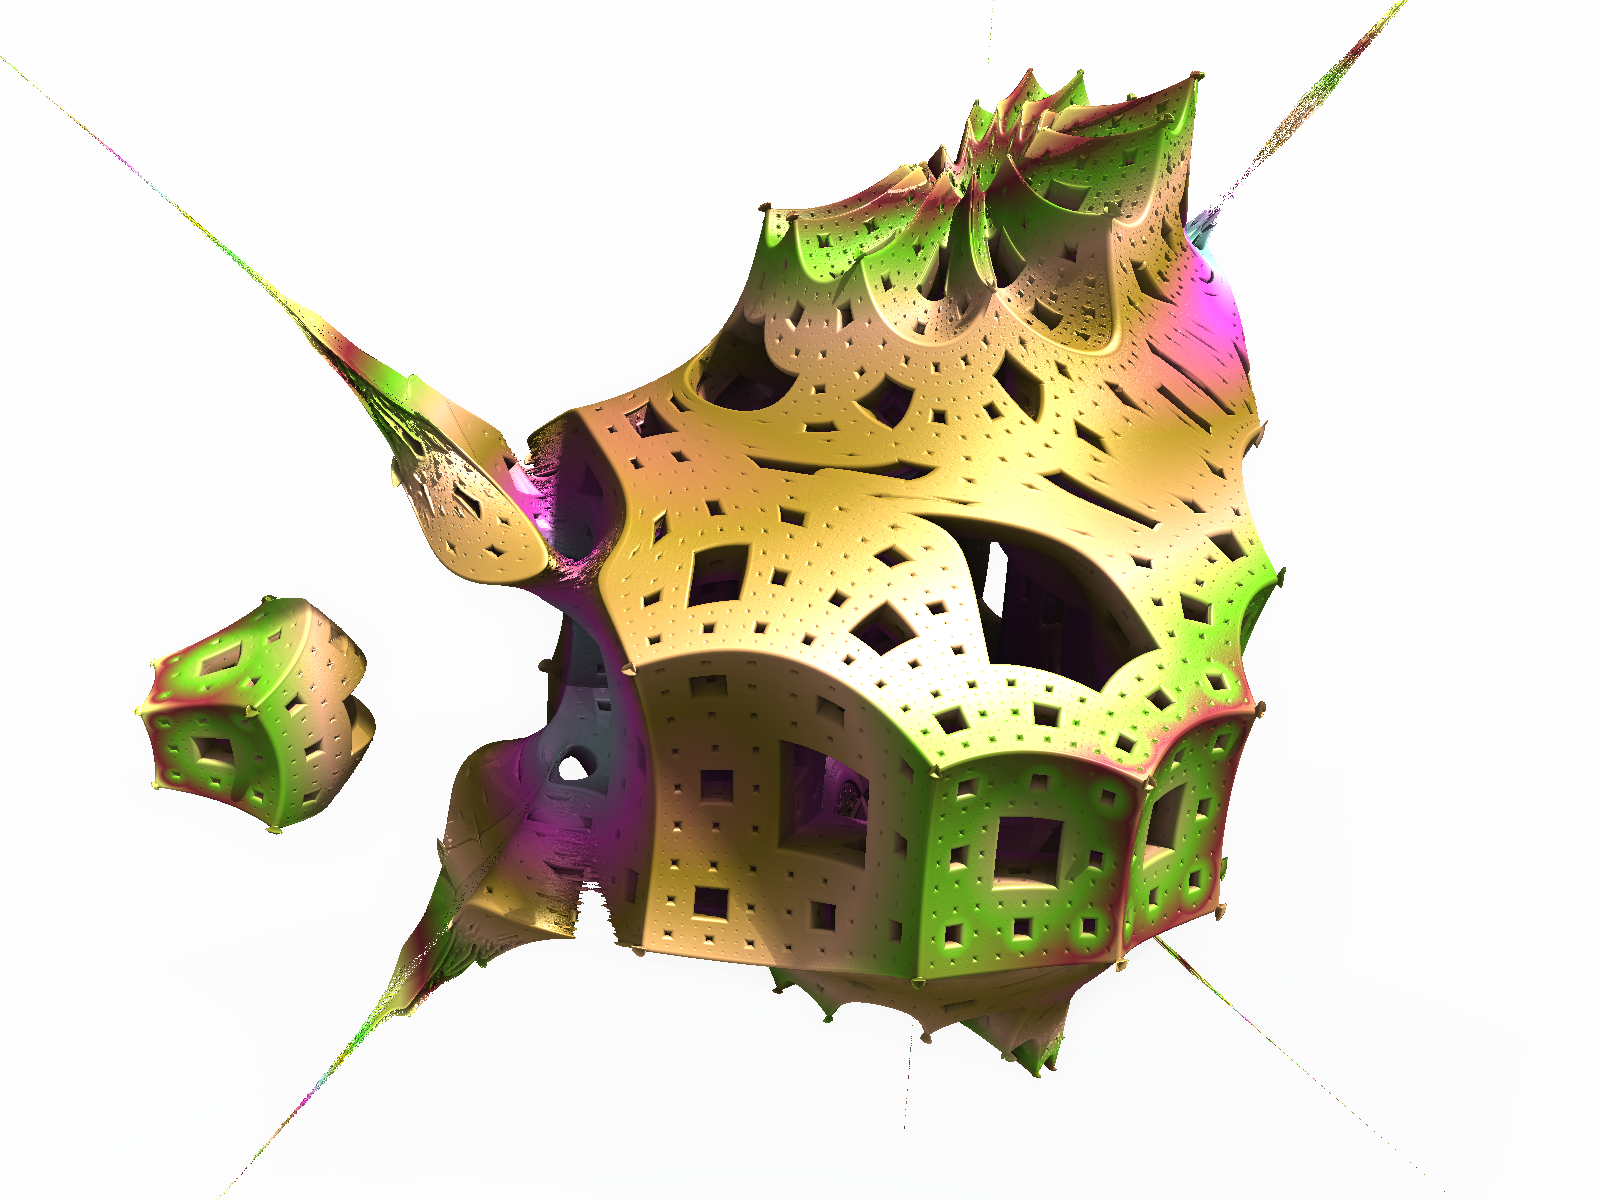
\includegraphics[width=0.7\linewidth]{img/manual/media/hybrid_sequence_example_3.png}

\subsubsection{Range of iterations for slot}

The sequence of fractal formulas can be configured more sophisticated.
It is possible to define a range of iterations on which a given formula will be used.

The second formula slot (\emph{Menger Sponge}) in the example below has the range of iterations set to \emph{from 4 to 250}.
On each tab the parameters \emph{Start at iteration} and {Stop at iteration} are used to define this range.

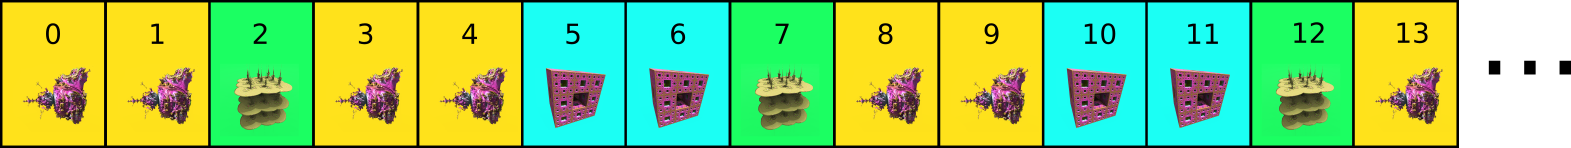
\includegraphics[width=\linewidth]{img/manual/media/iteration_loop_hybrid_sequence_4.png}

During the first pass of the sequence \emph{Menger Sponge} formula could be used at iterations 2 and 3.
Because \emph{Start at iteration} was 4 this formula slot was skipped.
During the second pass of the sequence \emph{Menger Sponge} formula was used at iterations 5 and 6,
because these iterations are inside the defined range of iterations.

The shape of the resulting fractal is the following:\nopagebreak

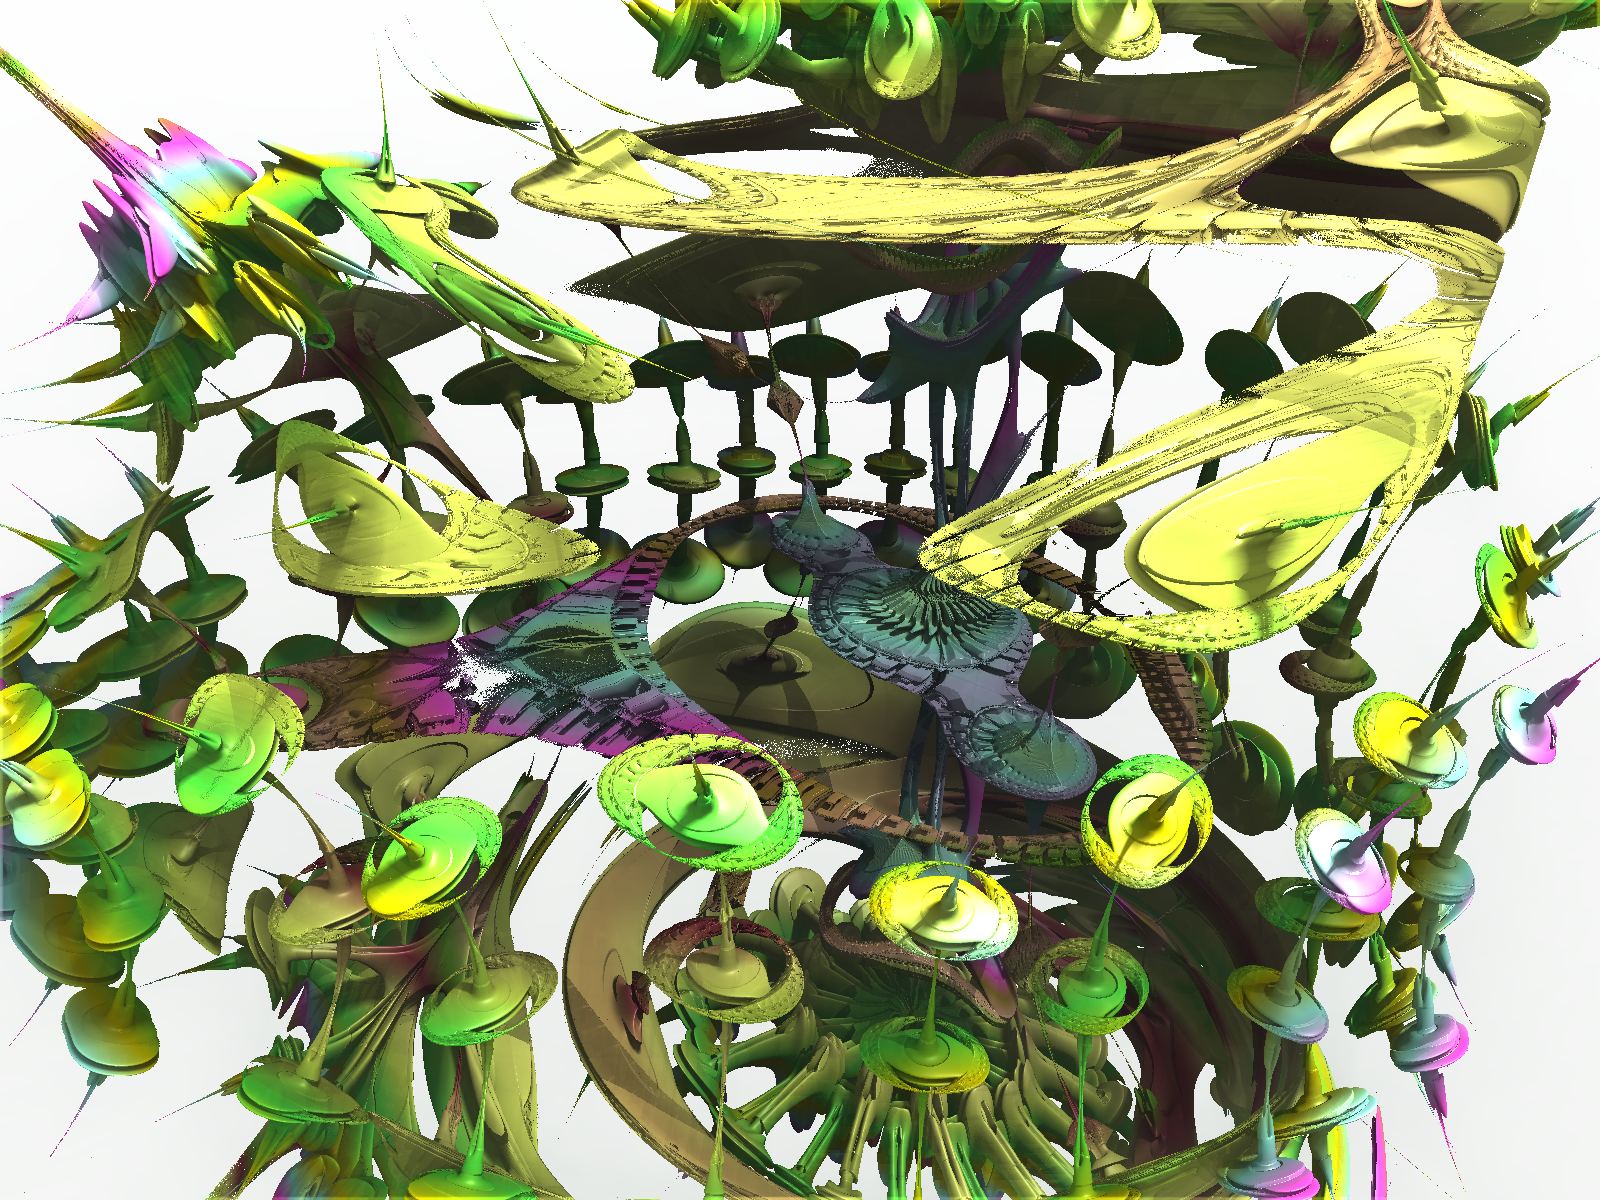
\includegraphics[width=0.7\linewidth]{img/manual/media/hybrid_sequence_example_4.png}

Because iteration number 2 is \emph{Box Fold Bulb Pow 2} formula the shape of it is much more visible.

\subsubsection{Changed order in sequence}

The order of fractal formulas can be easily changed with the use of the arrow buttons.

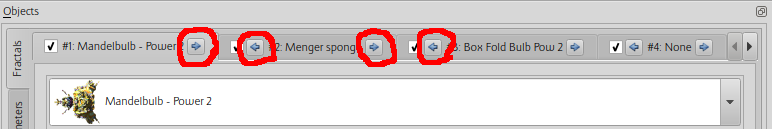
\includegraphics[width=\linewidth]{img/manual/media/fractal_tabs_with_defined_fractals_arrows.png}

Pressing these buttons causes swapping of fractal tabs and by that a swapping of the position inside the sequence.

Example based on first case showed in section \ref{two-iterations-per-slot}:
Swapped \emph{Mandelbulb - Power 2} and \emph{Menger Sponge} gives the following sequence:

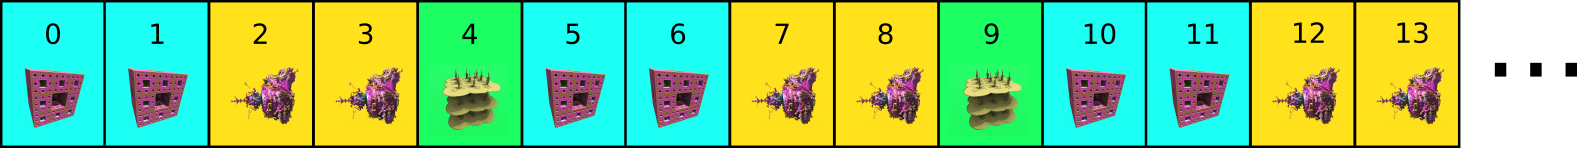
\includegraphics[width=\linewidth]{img/manual/media/iteration_loop_hybrid_sequence_5.png}

As visible in the image below, the shape of the fractal is completely different.\nopagebreak

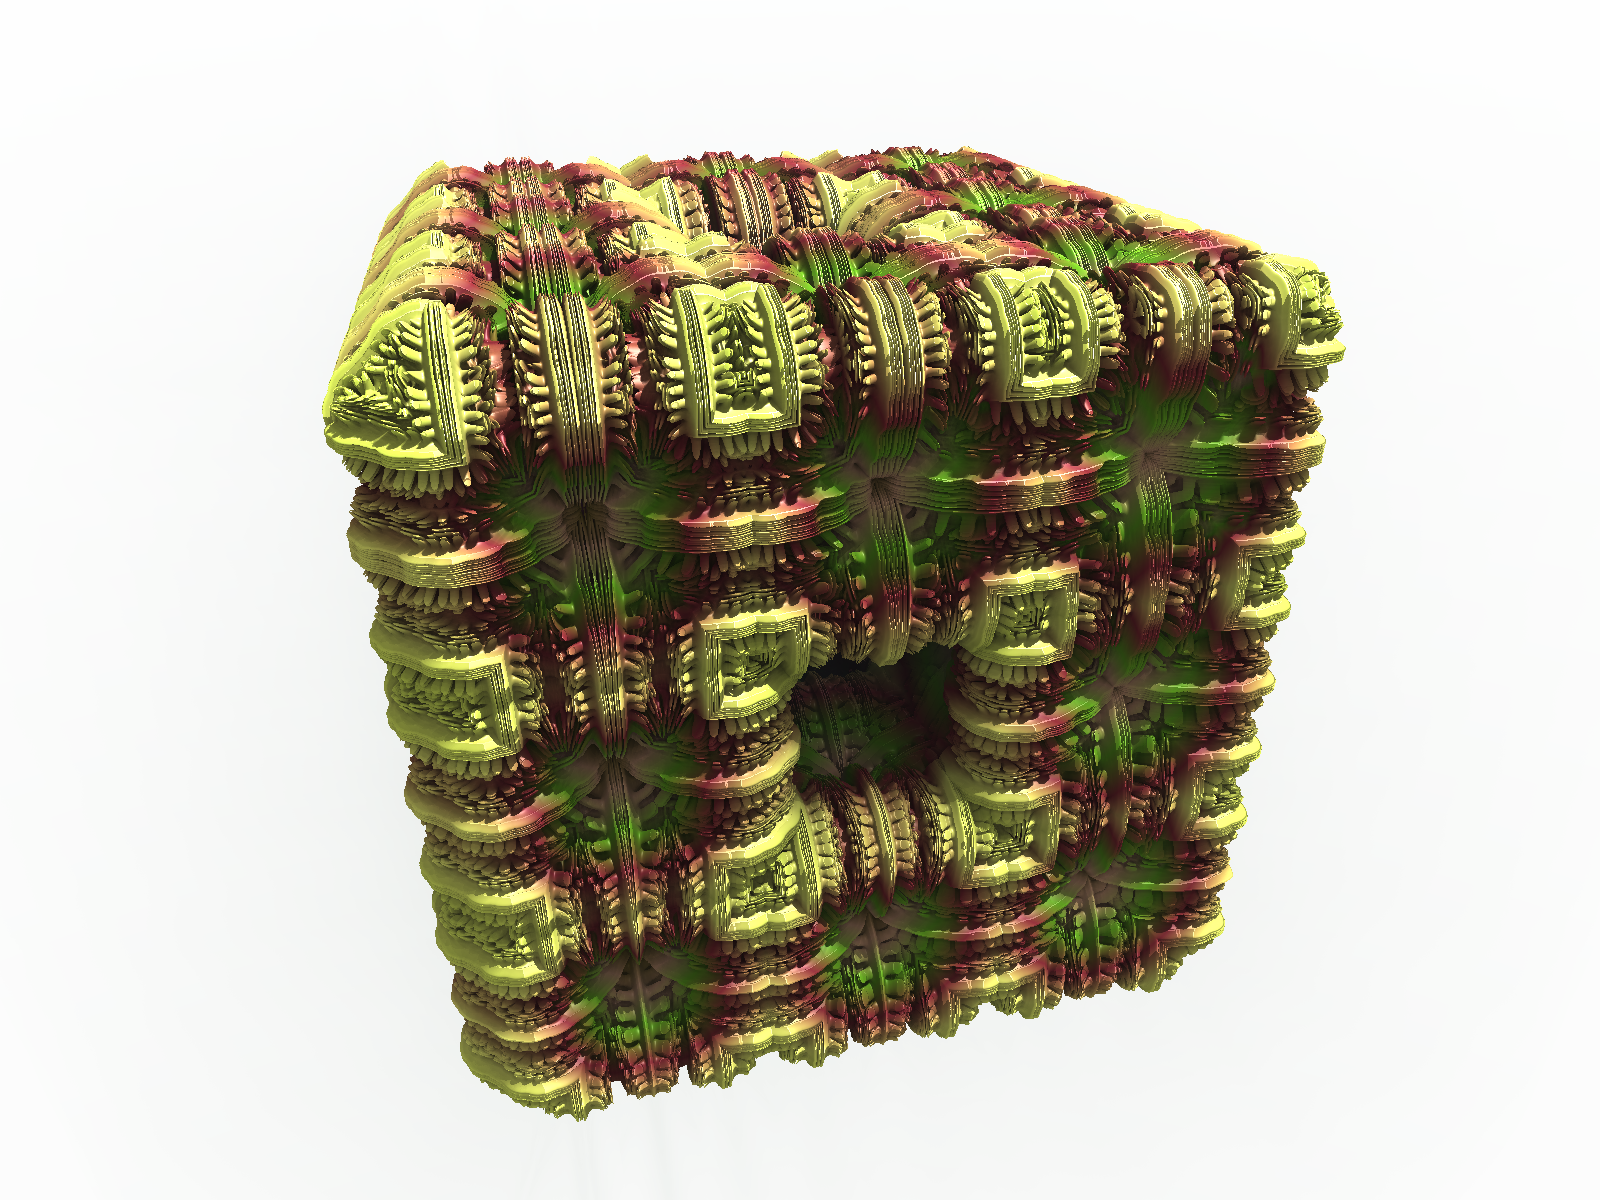
\includegraphics[width=0.7\linewidth]{img/manual/media/hybrid_sequence_example_5.png}

Even if the the same fractal formulas are used and in the same number of iterations per slot, the shape strongly depends on the order of the formulas.
Now first \emph{Menger Sponge} formula gives initial shape of fractal and \emph{Mandelbulb - Power 2} only modifies the details.
